
%% bare_conf.tex
%% V1.3
%% 2007/01/11
%% by Michael Shell
%% See:
%% http://www.michaelshell.org/
%% for current contact information.
%%
%% This is a skeleton file demonstrating the use of IEEEtran.cls
%% (requires IEEEtran.cls version 1.7 or later) with an IEEE conference paper.
%%
%% Support sites:
%% http://www.michaelshell.org/tex/ieeetran/
%% http://www.ctan.org/tex-archive/macros/latex/contrib/IEEEtran/
%% and
%% http://www.ieee.org/

%%*************************************************************************
%% Legal Notice:
%% This code is offered as-is without any warranty either expressed or
%% implied; without even the implied warranty of MERCHANTABILITY or
%% FITNESS FOR A PARTICULAR PURPOSE! 
%% User assumes all risk.
%% In no event shall IEEE or any contributor to this code be liable for
%% any damages or losses, including, but not limited to, incidental,
%% consequential, or any other damages, resulting from the use or misuse
%% of any information contained here.
%%
%% All comments are the opinions of their respective authors and are not
%% necessarily endorsed by the IEEE.
%%
%% This work is distributed under the LaTeX Project Public License (LPPL)
%% ( http://www.latex-project.org/ ) version 1.3, and may be freely used,
%% distributed and modified. A copy of the LPPL, version 1.3, is included
%% in the base LaTeX documentation of all distributions of LaTeX released
%% 2003/12/01 or later.
%% Retain all contribution notices and credits.
%% ** Modified files should be clearly indicated as such, including  **
%% ** renaming them and changing author support contact information. **
%%
%% File list of work: IEEEtran.cls, IEEEtran_HOWTO.pdf, bare_adv.tex,
%%                    bare_conf.tex, bare_jrnl.tex, bare_jrnl_compsoc.tex
%%*************************************************************************

% *** Authors should verify (and, if needed, correct) their LaTeX system  ***
% *** with the testflow diagnostic prior to trusting their LaTeX platform ***
% *** with production work. IEEE's font choices can trigger bugs that do  ***
% *** not appear when using other class files.                            ***
% The testflow support page is at:
% http://www.michaelshell.org/tex/testflow/



% Note that the a4paper option is mainly intended so that authors in
% countries using A4 can easily print to A4 and see how their papers will
% look in print - the typesetting of the document will not typically be
% affected with changes in paper size (but the bottom and side margins will).
% Use the testflow package mentioned above to verify correct handling of
% both paper sizes by the user's LaTeX system.
%
% Also note that the "draftcls" or "draftclsnofoot", not "draft", option
% should be used if it is desired that the figures are to be displayed in
% draft mode.
%
\documentclass[conference]{IEEEtran}
% Add the compsoc option for Computer Society conferences.
%
% If IEEEtran.cls has not been installed into the LaTeX system files,
% manually specify the path to it like:
% \documentclass[conference]{../sty/IEEEtran}





% Some very useful LaTeX packages include:
% (uncomment the ones you want to load)


% *** MISC UTILITY PACKAGES ***
%
%\usepackage{ifpdf}
% Heiko Oberdiek's ifpdf.sty is very useful if you need conditional
% compilation based on whether the output is pdf or dvi.
% usage:
% \ifpdf
%   % pdf code
% \else
%   % dvi code
% \fi
% The latest version of ifpdf.sty can be obtained from:
% http://www.ctan.org/tex-archive/macros/latex/contrib/oberdiek/
% Also, note that IEEEtran.cls V1.7 and later provides a builtin
% \ifCLASSINFOpdf conditional that works the same way.
% When switching from latex to pdflatex and vice-versa, the compiler may
% have to be run twice to clear warning/error messages.






% *** CITATION PACKAGES ***
%
%\usepackage{cite}
% cite.sty was written by Donald Arseneau
% V1.6 and later of IEEEtran pre-defines the format of the cite.sty package
% \cite{} output to follow that of IEEE. Loading the cite package will
% result in citation numbers being automatically sorted and properly
% "compressed/ranged". e.g., [1], [9], [2], [7], [5], [6] without using
% cite.sty will become [1], [2], [5]--[7], [9] using cite.sty. cite.sty's
% \cite will automatically add leading space, if needed. Use cite.sty's
% noadjust option (cite.sty V3.8 and later) if you want to turn this off.
% cite.sty is already installed on most LaTeX systems. Be sure and use
% version 4.0 (2003-05-27) and later if using hyperref.sty. cite.sty does
% not currently provide for hyperlinked citations.
% The latest version can be obtained at:
% http://www.ctan.org/tex-archive/macros/latex/contrib/cite/
% The documentation is contained in the cite.sty file itself.






% *** GRAPHICS RELATED PACKAGES ***
%
\ifCLASSINFOpdf
   \usepackage[pdftex]{graphicx}
  % declare the path(s) where your graphic files are
   \graphicspath{{../pdf/}{../jpeg/}}
  % and their extensions so you won't have to specify these with
  % every instance of \includegraphics
   \DeclareGraphicsExtensions{.pdf,.jpeg,.png}
\else
  % or other class option (dvipsone, dvipdf, if not using dvips). graphicx
  % will default to the driver specified in the system graphics.cfg if no
  % driver is specified.
   \usepackage[dvips]{graphicx}
  % declare the path(s) where your graphic files are
   \graphicspath{{./}}
  % and their extensions so you won't have to specify these with
  % every instance of \includegraphics
%   \DeclareGraphicsExtensions{.eps}
\fi
% graphicx was written by David Carlisle and Sebastian Rahtz. It is
% required if you want graphics, photos, etc. graphicx.sty is already
% installed on most LaTeX systems. The latest version and documentation can
% be obtained at: 
% http://www.ctan.org/tex-archive/macros/latex/required/graphics/
% Another good source of documentation is "Using Imported Graphics in
% LaTeX2e" by Keith Reckdahl which can be found as epslatex.ps or
% epslatex.pdf at: http://www.ctan.org/tex-archive/info/
%
% latex, and pdflatex in dvi mode, support graphics in encapsulated
% postscript (.eps) format. pdflatex in pdf mode supports graphics
% in .pdf, .jpeg, .png and .mps (metapost) formats. Users should ensure
% that all non-photo figures use a vector format (.eps, .pdf, .mps) and
% not a bitmapped formats (.jpeg, .png). IEEE frowns on bitmapped formats
% which can result in "jaggedy"/blurry rendering of lines and letters as
% well as large increases in file sizes.
%
% You can find documentation about the pdfTeX application at:
% http://www.tug.org/applications/pdftex


\usepackage{epstopdf}


% *** MATH PACKAGES ***
%
\usepackage[cmex10]{amsmath}
% A popular package from the American Mathematical Society that provides
% many useful and powerful commands for dealing with mathematics. If using
% it, be sure to load this package with the cmex10 option to ensure that
% only type 1 fonts will utilized at all point sizes. Without this option,
% it is possible that some math symbols, particularly those within
% footnotes, will be rendered in bitmap form which will result in a
% document that can not be IEEE Xplore compliant!
%
% Also, note that the amsmath package sets \interdisplaylinepenalty to 10000
% thus preventing page breaks from occurring within multiline equations. Use:
%\interdisplaylinepenalty=2500
% after loading amsmath to restore such page breaks as IEEEtran.cls normally
% does. amsmath.sty is already installed on most LaTeX systems. The latest
% version and documentation can be obtained at:
% http://www.ctan.org/tex-archive/macros/latex/required/amslatex/math/





% *** SPECIALIZED LIST PACKAGES ***
%
%\usepackage{algorithmic}
% algorithmic.sty was written by Peter Williams and Rogerio Brito.
% This package provides an algorithmic environment fo describing algorithms.
% You can use the algorithmic environment in-text or within a figure
% environment to provide for a floating algorithm. Do NOT use the algorithm
% floating environment provided by algorithm.sty (by the same authors) or
% algorithm2e.sty (by Christophe Fiorio) as IEEE does not use dedicated
% algorithm float types and packages that provide these will not provide
% correct IEEE style captions. The latest version and documentation of
% algorithmic.sty can be obtained at:
% http://www.ctan.org/tex-archive/macros/latex/contrib/algorithms/
% There is also a support site at:
% http://algorithms.berlios.de/index.html
% Also of interest may be the (relatively newer and more customizable)
% algorithmicx.sty package by Szasz Janos:
% http://www.ctan.org/tex-archive/macros/latex/contrib/algorithmicx/




% *** ALIGNMENT PACKAGES ***
%
%\usepackage{array}
% Frank Mittelbach's and David Carlisle's array.sty patches and improves
% the standard LaTeX2e array and tabular environments to provide better
% appearance and additional user controls. As the default LaTeX2e table
% generation code is lacking to the point of almost being broken with
% respect to the quality of the end results, all users are strongly
% advised to use an enhanced (at the very least that provided by array.sty)
% set of table tools. array.sty is already installed on most systems. The
% latest version and documentation can be obtained at:
% http://www.ctan.org/tex-archive/macros/latex/required/tools/


%\usepackage{mdwmath}
%\usepackage{mdwtab}
% Also highly recommended is Mark Wooding's extremely powerful MDW tools,
% especially mdwmath.sty and mdwtab.sty which are used to format equations
% and tables, respectively. The MDWtools set is already installed on most
% LaTeX systems. The lastest version and documentation is available at:
% http://www.ctan.org/tex-archive/macros/latex/contrib/mdwtools/


% IEEEtran contains the IEEEeqnarray family of commands that can be used to
% generate multiline equations as well as matrices, tables, etc., of high
% quality.


%\usepackage{eqparbox}
% Also of notable interest is Scott Pakin's eqparbox package for creating
% (automatically sized) equal width boxes - aka "natural width parboxes".
% Available at:
% http://www.ctan.org/tex-archive/macros/latex/contrib/eqparbox/





% *** SUBFIGURE PACKAGES ***
%\usepackage[tight,footnotesize]{subfigure}
% subfigure.sty was written by Steven Douglas Cochran. This package makes it
% easy to put subfigures in your figures. e.g., "Figure 1a and 1b". For IEEE
% work, it is a good idea to load it with the tight package option to reduce
% the amount of white space around the subfigures. subfigure.sty is already
% installed on most LaTeX systems. The latest version and documentation can
% be obtained at:
% http://www.ctan.org/tex-archive/obsolete/macros/latex/contrib/subfigure/
% subfigure.sty has been superceeded by subfig.sty.



%\usepackage[caption=false]{caption}
%\usepackage[font=footnotesize]{subfig}
% subfig.sty, also written by Steven Douglas Cochran, is the modern
% replacement for subfigure.sty. However, subfig.sty requires and
% automatically loads Axel Sommerfeldt's caption.sty which will override
% IEEEtran.cls handling of captions and this will result in nonIEEE style
% figure/table captions. To prevent this problem, be sure and preload
% caption.sty with its "caption=false" package option. This is will preserve
% IEEEtran.cls handing of captions. Version 1.3 (2005/06/28) and later 
% (recommended due to many improvements over 1.2) of subfig.sty supports
% the caption=false option directly:
%\usepackage[caption=false,font=footnotesize]{subfig}
%
% The latest version and documentation can be obtained at:
% http://www.ctan.org/tex-archive/macros/latex/contrib/subfig/
% The latest version and documentation of caption.sty can be obtained at:
% http://www.ctan.org/tex-archive/macros/latex/contrib/caption/




% *** FLOAT PACKAGES ***
%
%\usepackage{fixltx2e}
% fixltx2e, the successor to the earlier fix2col.sty, was written by
% Frank Mittelbach and David Carlisle. This package corrects a few problems
% in the LaTeX2e kernel, the most notable of which is that in current
% LaTeX2e releases, the ordering of single and double column floats is not
% guaranteed to be preserved. Thus, an unpatched LaTeX2e can allow a
% single column figure to be placed prior to an earlier double column
% figure. The latest version and documentation can be found at:
% http://www.ctan.org/tex-archive/macros/latex/base/



%\usepackage{stfloats}
% stfloats.sty was written by Sigitas Tolusis. This package gives LaTeX2e
% the ability to do double column floats at the bottom of the page as well
% as the top. (e.g., "\begin{figure*}[!b]" is not normally possible in
% LaTeX2e). It also provides a command:
%\fnbelowfloat
% to enable the placement of footnotes below bottom floats (the standard
% LaTeX2e kernel puts them above bottom floats). This is an invasive package
% which rewrites many portions of the LaTeX2e float routines. It may not work
% with other packages that modify the LaTeX2e float routines. The latest
% version and documentation can be obtained at:
% http://www.ctan.org/tex-archive/macros/latex/contrib/sttools/
% Documentation is contained in the stfloats.sty comments as well as in the
% presfull.pdf file. Do not use the stfloats baselinefloat ability as IEEE
% does not allow \baselineskip to stretch. Authors submitting work to the
% IEEE should note that IEEE rarely uses double column equations and
% that authors should try to avoid such use. Do not be tempted to use the
% cuted.sty or midfloat.sty packages (also by Sigitas Tolusis) as IEEE does
% not format its papers in such ways.





% *** PDF, URL AND HYPERLINK PACKAGES ***
%
%\usepackage{url}
% url.sty was written by Donald Arseneau. It provides better support for
% handling and breaking URLs. url.sty is already installed on most LaTeX
% systems. The latest version can be obtained at:
% http://www.ctan.org/tex-archive/macros/latex/contrib/misc/
% Read the url.sty source comments for usage information. Basically,
% \url{my_url_here}.





% *** Do not adjust lengths that control margins, column widths, etc. ***
% *** Do not use packages that alter fonts (such as pslatex).         ***
% There should be no need to do such things with IEEEtran.cls V1.6 and later.
% (Unless specifically asked to do so by the journal or conference you plan
% to submit to, of course. )


% correct bad hyphenation here
\hyphenation{op-tical net-works semi-conduc-tor}


\begin{document}
%
% paper title
% can use linebreaks \\ within to get better formatting as desired
\title{Motor Experience Alters Action Perception Through Predictive Learning of Sensorimotor Information}

% author names and affiliations
% use a multiple column layout for up to three different
% affiliations
\author{\IEEEauthorblockN{Jimmy Baraglia, Jorge L. Copete, Yukie Nagai, Minoru Asada}
\IEEEauthorblockA{Graduate School of Engineering, Osaka University\\
Japan, Osaka, Suita, Yamadaoka, 2-1, U1W-618 \\
Email: jimmy.baraglia@ams.eng.osaka-u.ac.jp}
%\and
%\IEEEauthorblockN{Homer Simpson}
%\IEEEauthorblockA{Twentieth Century Fox\\
%Springfield, USA\\
%Email: homer@thesimpsons.com}
}

% conference papers do not typically use \thanks and this command
% is locked out in conference mode. If really needed, such as for
% the acknowledgment of grants, issue a \IEEEoverridecommandlockouts
% after \documentclass

% for over three affiliations, or if they all won't fit within the width
% of the page, use this alternative format:
% 
%\author{\IEEEauthorblockN{Michael Shell\IEEEauthorrefmark{1},
%Homer Simpson\IEEEauthorrefmark{2},
%James Kirk\IEEEauthorrefmark{3}, 
%Montgomery Scott\IEEEauthorrefmark{3} and
%Eldon Tyrell\IEEEauthorrefmark{4}}
%\IEEEauthorblockA{\IEEEauthorrefmark{1}School of Electrical and Computer Engineering\\
%Georgia Institute of Technology,
%Atlanta, Georgia 30332--0250\\ Email: see http://www.michaelshell.org/contact.html}
%\IEEEauthorblockA{\IEEEauthorrefmark{2}Twentieth Century Fox, Springfield, USA\\
%Email: homer@thesimpsons.com}
%\IEEEauthorblockA{\IEEEauthorrefmark{3}Starfleet Academy, San Francisco, California 96678-2391\\
%Telephone: (800) 555--1212, Fax: (888) 555--1212}
%\IEEEauthorblockA{\IEEEauthorrefmark{4}Tyrell Inc., 123 Replicant Street, Los Angeles, California 90210--4321}}




% use for special paper notices
%\IEEEspecialpapernotice{(Invited Paper)}


% make the title area
\maketitle

\begin{abstract}
%\boldmath
Recent studies have revealed that infants' goal-directed-actions execution strongly alters their perception of similar actions performed by others. Such an ability to recognize correspondences between self-experience and others' actions may be crucial for the development of higher cognitive social skills. However, there is not yet a computational model or constructive explanation accounting for the role of action generation in the perception of others' actions. To address this issue, we hypothesize that the sensory and motor information are integrated at a neural level through a predictive learning process that combines both modalities. Thus, the experience of motor actions alters the representation of the sensorimotor integration, which causes changes in the perception of others' actions. To test this hypothesis, we built a computational model that integrates visual and motor (hereafter, visuomotor) information using a Recurrent Neural Network (RNN) which is capable of learning temporal sequences of data. We modeled the visual attention of the system based on a prediction error between the visuomotor prediction and the actual visuomotor values, which maximizes the attention toward not too predictable and not too unpredictable sensory information. We performed a series of experiments with a simulated humanoid robot from which we observed that motor activation during self-generated actions biased the robot's perception of others' actions. These results highlight the important role of modalities integration in humans, which accounts for a biased perception of our environment based on a restricted repertoire of own experienced actions.

\end{abstract}
% IEEEtran.cls defaults to using nonbold math in the Abstract.
% This preserves the distinction between vectors and scalars. However,
% if the conference you are submitting to favors bold math in the abstract,
% then you can use LaTeX's standard command \boldmath at the very start
% of the abstract to achieve this. Many IEEE journals/conferences frown on
% math in the abstract anyway.

% no keywords

% For peer review papers, you can put extra information on the cover
% page as needed:
% \ifCLASSOPTIONpeerreview
% \begin{center} \bfseries EDICS Category: 3-BBND \end{center}
% \fi
%
% For peerreview papers, this IEEEtran command inserts a page break and
% creates the second title. It will be ignored for other modes.
\IEEEpeerreviewmaketitle


\section{Introduction}
% no \IEEEPARstart
In early infancy, humans are not yet able to detect the goal of others' actions. Later on, infants undergo a developmental process that allows us to perceive others' actions as goal-directed. Several studies have been carried out to reveal when and how infants start understanding goal-directed actions. A remarkable work conducted by Woodward \cite{woodward1998infants} shows that infants (5, 6 and 9 months old) with goal-directed action experience react differently to actors reaching for and grasping objects. For the experiments four actors were presented to the infants: a human arm, a rod, a flat occluder and a mechanical grasping tool. The experiment indicated that when infants were habituated to goal-directed actions (i.e., the human arm condition) they showed a stronger novelty response to test events that varied the goal of the action (e.g., the grasped object) than test events that varied the physical properties of the action (e.g., the motion path). On the other hand, if the actions were not goal-directed (i.e., the rod and the flat occluder conditions), or were goal-directed but difficult to infer the agency of the actor (i.e., the mechanical grasping tool condition), infants did not prefer one type of response to the other (i.e., the goal of the action versus the properties of the action).

Later, Sommerville et al.\cite{sommerville2005action} studied the impact of infants' action production in perception of others' actions. The participants of the experiment were 3-month-old infants. They were divided in two groups. The first group of infants participated in an action task which consisted in getting action experience by interacting with two objects. The second group did not participant in the action task. Due to the fact that 3-month-old infants are not yet able to perform coordinated gaze and manual contact with objects, they put a pair of mittens on the infants’ hands so that they can easily make contact with them. Then, during the habituation phase, both groups of infants saw an actor reach for and grasp one of two objects. Finally, during the test phase, the position of the objects was reversed and the infants saw new test events: a new goal event (e.g., the actor reached the same position as habituation but grasped a different goal), and a new path event (e.g., the actor reached a different position but grasped the same goal). Infants' looking time was measured during the experiment. The results showed that the looking time of the first group of infants was longer than the looking time of the second group in the first trial of the habituation phase. The results also showed that the first group of infants looked significantly longer at the new goal event than the new path event, whereas the second group of infants looked equally to both events. In authors' view, these findings reflect infants’ ability to detect the goal structure of action after experiencing object-directed behavior, and to apply this knowledge when perceiving others’ actions. Also that self-action production may provide increased impetus to attend to action goals. From this study we found that in order to understand this phenomenon, it is important to clarify how motor and visual systems interact with each other, and to explain how they influence visual attention.

Among works explaining relevant phenomenon regarding allocation of visual attention, a significant study conducted by Kidd et al. \cite{kidd2012goldilocks} measured 7- and 8-month-old infants attention when varying the complexity of a sequence of visual events. The experiments showed that the probability of infants to look away from events became higher when the complexity of the stimulus was very low or very high. They suggested that infants allocate their attention in order to maintain an intermediate level of complexity.

In this study we build a computational model to explain how action production alters perception of others’ actions as reported by Sommerville et al. \cite{sommerville2005action}. Specifically, we focus on the relation between the visual and motor systems and the effect of action experience on the perception of others’ action. Our hypothesis is that motor activity biases visual perception through the joint representation of visuomotor experiences. As an extension to the aforementioned hypothesis, we also propose that the allocation of visual attention is modulated by the prediction error that results from making correspondence between own experience and others' actions. We carried out experiments using iCub Simulator to validate our hypothesis.

\section{Hypothesis}
 
\subsection{Findings in Infant Study}
Sommerville et al. \cite{sommerville2005action} reported that infants' action experience alters their perception when observing others' actions. Here we focused on two main findings:
 
\begin{enumerate}
\item Experience apprehending objects initially increases infants’ attention to similar reaching events performed by another person (Figure 2 in \cite{sommerville2005action});
\item Infants with apprehension experience look significantly longer at new goal events than new path events, whereas infants without that experience looked equally to both events (Figure 3 in \cite{sommerville2005action}).
\end{enumerate}
 
Sommerville et al. \cite{sommerville2005action} suggested that the first finding "may reflect infants’ ability to recognize correspondences across executed and observed actions and/or an increased motivation to attend to action after acting". Regarding the second finding, they indicated that "experience apprehending objects directly prior to viewing the visual habituation event enabled infants to detect the goal-directed structure of the event in another person's actions".

\subsection{Our Hypothesis}
We argue that action experience is acquired through the process of integrating motor and sensory information, and that the joint representation derived from this integration is used to learn to predict other's actions. Based on this argumentation, our hypothesis is that the motor experience of goal-directed actions biases our sensorimotor representation, and this alteration causes a change in the prediction of sensorial information when observing others' actions.

During this learning process a prediction error arises between the predicted sensorimotor information and the actual sensory value. The magnitude of the prediction error depends on the action experience. We hypothesize that the prediction error modulates the level of interest to external stimulus so that moderate prediction errors (e.g., not too high and not too low) elicit an increase of infants’ interest. Regarding this idea, we adopt the evidence in \cite{kidd2012goldilocks} according to which visual allocation depends on the complexity of the events, where scenes of middle level complexity draw more attention than those of low and high levels.

We explain findings in \cite{sommerville2005action} in correspondence to our hypothesis saying that when infants acquire motor experience their joint representation of sensorimotor experience changes, which alters how they predict sensorial information from new events. Then, the attention of infants increases and reaches the highest value when the prediction error of new events is moderate. As a consequence:

\begin{enumerate}
\item When infants have experience apprehending objects the prediction error increases but reaches a moderate value if they observe similar reaching events performed by another person, which explains why infants’ attention increased more in the case of infants with action experience than of infants without action experience.
\item Experience apprehending objects (e.g., goal-directed action experience) enables infants to learn to distinguish between goal and trajectory, which makes the prediction error to keep low if the trajectory changes when observing reaching events to the same goal, and to increase but to a moderate value if the goal changes but the trajectory keeps the same. This explains why infants looked significantly longer at new goal events than new path events. On the other hand, infants without that experience lack of such a kind of distinction, which makes their prediction error to become high for new path events and low for new goal events. Therefore, they looked equally to both events.
\end{enumerate}

\section{Computational Model}
We propose a computational model based on our hypothesis, as shown in Fig. 1. First, the visual module extracts the visual positions and relations of the objects in the scene. The motor module generates the motor primitives and the motion target of an action. Then, the sensorimotor integration and predictive learning module integrates and learns to predict the visuomotor information. Finally, the visual attention module employs the prediction error to calculate the interest function which in inversely proportional to the probability of looking away from an event. The details of each module are explained in following subsections.

\begin{figure}
\centering
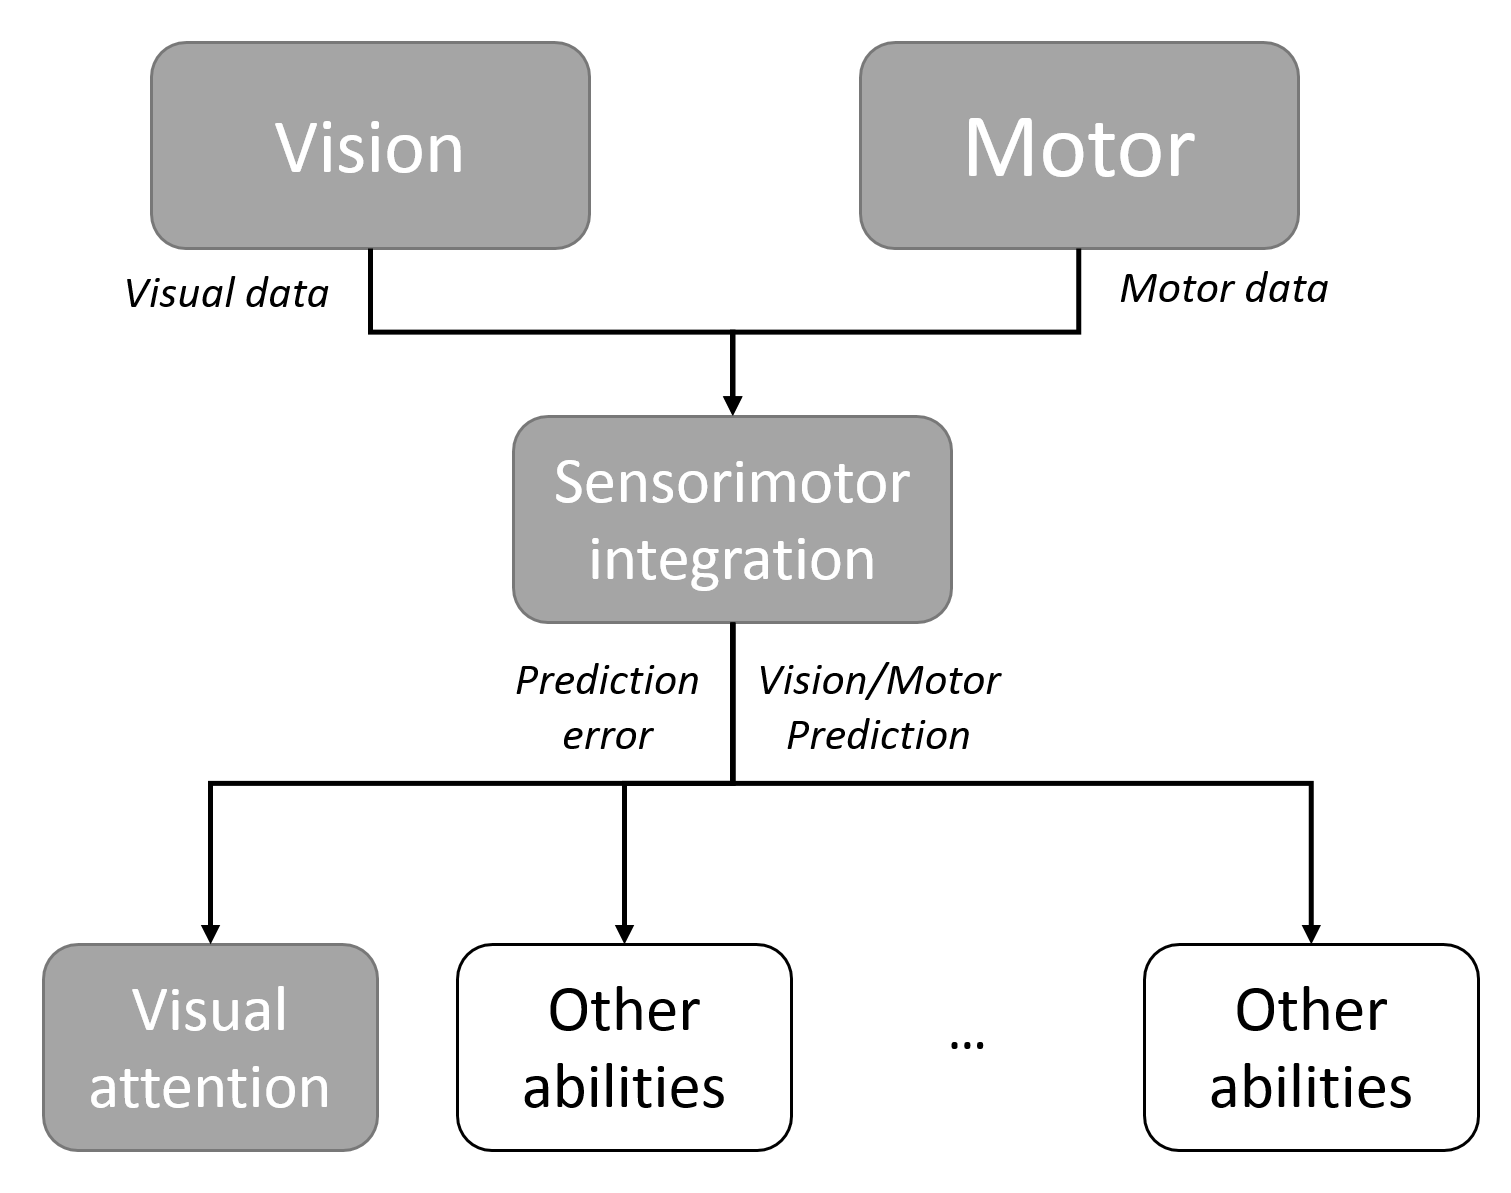
\includegraphics[width=0.45\textwidth,natwidth=700,natheight=450]{Figure1.png}
\caption{Proposed computational model for visual attention}
\label{figure1}
\end{figure}

\subsection{Motor Module}
The motor module generates motor activation signals when the system performs actions. Here, we represent the motor activity as a distinctive set of signals which encode the target of the action and the motor primitive currently generated. This module will output:
\begin{itemize}
\item The motor primitives represented as a vector of $k$ binary neurons, where $k$ is the number of action primitives.
\item The target of the ongoing action as a vector of $n$ binary and mutually exclusive neurons, where $n$ is the number of objects in the scene.
\end{itemize}
For the case of a scene composed of two objects ($k$=2) with two motor primitives ($n$=2), arm reaching primitive and arm retracting primitive, the motor module will output a vector \text{M} composed of four activations signals,
\begin{equation}
	\textbf{M}(t)=[\text{P}_{1}(t), \text{P}_{2}(t), \text{G}_{1}(t), \text{G}_{2}(t)],
\end{equation}
where \(\text{G}_{1}\), \(\text{G}_{2}\) take values 0 or 1, are mutually exclusive and represent the two targets present in our scene, and \(\text{P}_{1}(t), \text{P}_{2}(t)\) take values 0 or 1 and represent the activation of two action primitives.

\subsection{Vision Module}
The vision module extracts visual information when the system observes actions and provides information of the position of the moving effector, and the relations between objects in the scene: getting closer or getting away. To do so, the module first extracts and tracks the objects in the scene, then measures their relative dynamic and finally employs the resulting motion vectors to calculate their relations. For the case of a scene composed of two fixed objects and one moving agent, the output of the vision module is the vector \(\text{V}\). The structure of a vector \(\text{V}\) is as follows,

\begin{equation}
\begin{split}
	\textbf{V}(t)=[\text{x}(t), \text{y}(t), \text{z}(t), \text{R}_{11}(t), \text{R}_{12}(t),\\ \text{R}_{21}(t), \text{R}_{22}(t), \text{RG}_{1}(t), \text{RG}_{2}(t)],
\end{split}
\end{equation}
where $x$, $y$ and $z$ represent the visual position of the hand, \(\text{R}_{11}\), \(\text{R}_{12}\) and \(\text{R}_{21}\), \(\text{R}_{22}\) take values 0 or 1 and represent the four possible relations between two objects and the agent: agent getting closer to object 1, agent getting away from object 2, agent getting closer to object 2, and agent getting away from object 2, respectively. \(\text{RG}_{1}\), \(\text{RG}_{2}\) represent the global relations independent of the target object: agent getting closer to an object and agent getting away from an object, respectively.

\subsection{Sensorimotor Integration and Predictive Learning Module}
\subsubsection{Sensorimotor Integration and Predictive Learning}
Biological systems use multiple sensorimotor modalities to interact with their environment. We argue that the process of integrating multi-modal information, such as visual and motor information, contributes to encode our experience and is vital to understand others' action goals. For that purpose, we take advantage of the structure and functionality of the Elman Recurrent Neural Network (RNN) \cite{elman1990finding} which can perform integration of multiple data and learn the characteristic of temporal sequence data. The model of the neural network is shown in Fig. \ref{NeuralNet}. The inputs of the neural network \(\textbf{I}(t)\) are the outputs from the visual module and the motor module,

\begin{equation}
	\textbf{I}(t)=[\textbf{V}(t), \textbf{M}(t)],\\
\end{equation}
and the outputs \(\textbf{O}(t)\) are the predicted visual and motor data,
\begin{equation}
	\textbf{O}(t+1)=[\hat{\textbf{V}}(t+1), \hat{\textbf{M}}(t+1)],\\
\end{equation}
where \(\hat{\textbf{V}}(t)\) is the predicted visual information, and  \(\hat{\textbf{M}}(t)\) is the predicted motor information. The internal composition of \(\hat{\textbf{V}}(t)\) and \(\hat{\textbf{M}}(t)\) is equivalent to \(\text{\textbf{V}}(t)\) and \(\text{\textbf{M}}(t)\), respectively. The neural network is trained using the back propagation through time method to minimize the learning error which considers sensory-based and motor-based errors.

\begin{figure}[!t]
\centering
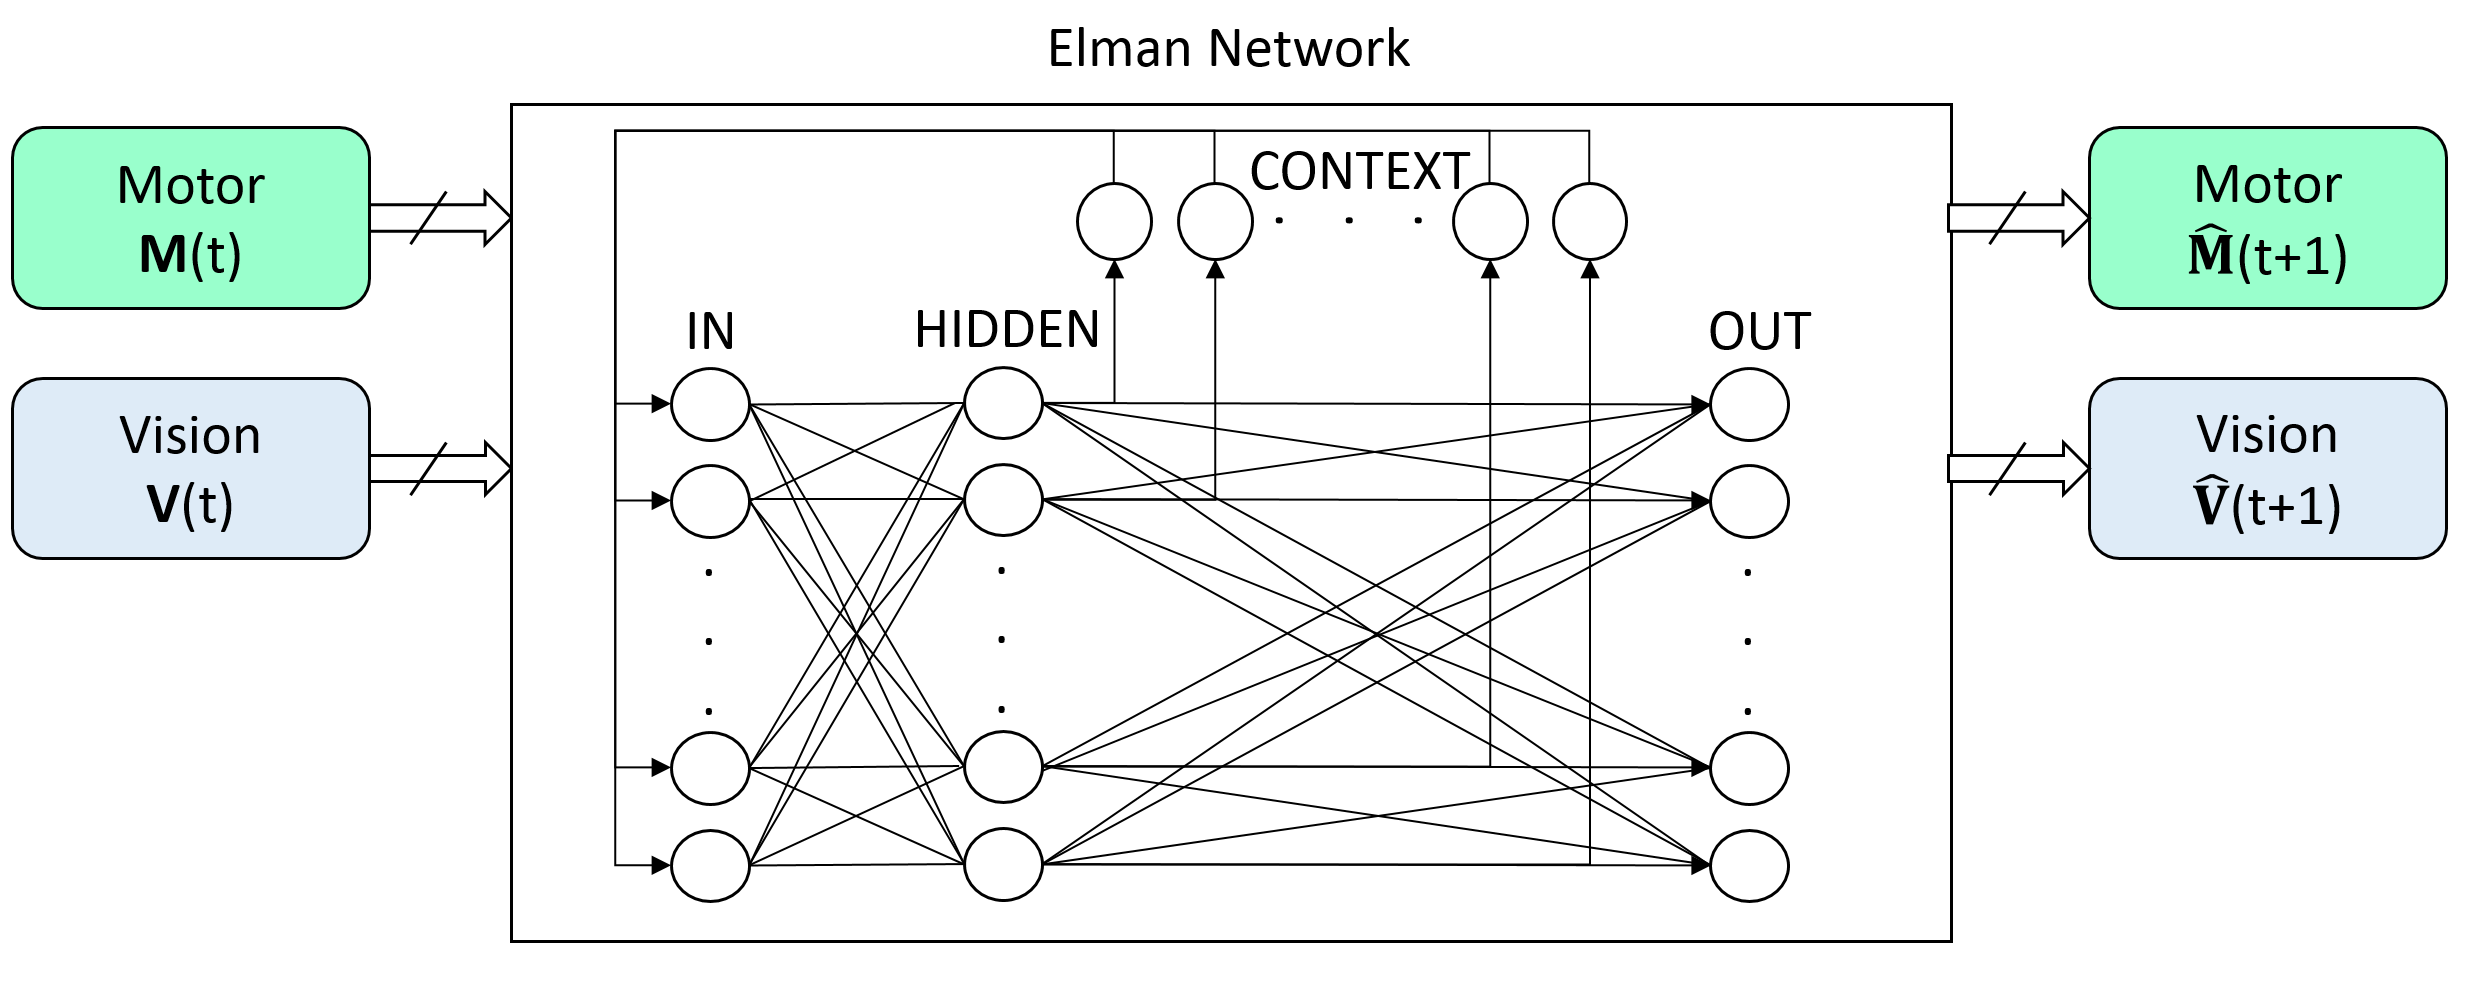
\includegraphics[width=0.5\textwidth,natwidth=700,natheight=450]{Elman_Network.png}
\caption{Internal structure of the sensorimotor integration module based on a Recurrent Neural Network}
\label{NeuralNet}
\end{figure}

\subsubsection{Prediction Error}
Humans tend to anticipate near future events when interacting with the environment based on the sensory data they perceive. However, humans' capacity to make predictions is strongly influenced by our experience, and the lack of experience makes the prediction outcome when observing others' actions differs largely from the actual outcome. We define this difference as prediction error. We argue that the prediction error plays a fundamental role in the development of several cognitive abilities. The prediction error \(\text{E}(t+1)\) is calculated as,

\begin{equation}
\begin{split}
	\text{E}(t+1)=|\hat{\textbf{V}}(t+1)-\text{\textbf{V}}(t+1)|,\\
\end{split}
\end{equation}
where \(\hat{\textbf{V}}(t+1)\)  is the predicted sensory data, and \(\text{\textbf{V}}(t+1)\) is the actual sensory data.

\subsection{Visual Attention Module}
For implementing the visual attention module we adopted the findings of Kidd et al. \cite{kidd2012goldilocks} who suggested that infants allocate their attention in order to maintain an intermediate level of complexity. Hereafter we will refer to this as the principle of predictability, where the complexity is represented by the prediction error. The probability \(\text{A}\) of looking away from the current visual position is proportional to an interest function \(\text{N}\),

\begin{equation}
  \text{A}(t) = 1 - \alpha\cdot\text{N},
\end{equation}
\begin{equation}
  \text{N}(t) = \frac{1}{\sigma\cdot \sqrt{2\cdot\pi}}\cdot e^{\frac{-(E-U)^2}{2\cdot\sigma^2}}
  \label{gaussian}
\end{equation}
where \(\alpha\) is a scaling factor, and \(\sigma\) and \(\text{U}\) are the variance and mean value of the prediction error, respectively. The interest function \(\text{N}\) and the probability of looking away \(\text{A}\) are shown in Fig. \ref{Attention}, where the interest function is maximized when the observed action is not too predictable (i.e. prediction error is too low) or too unpredictable (i.e., prediction error is too high).

\begin{figure}[!t]
\centering
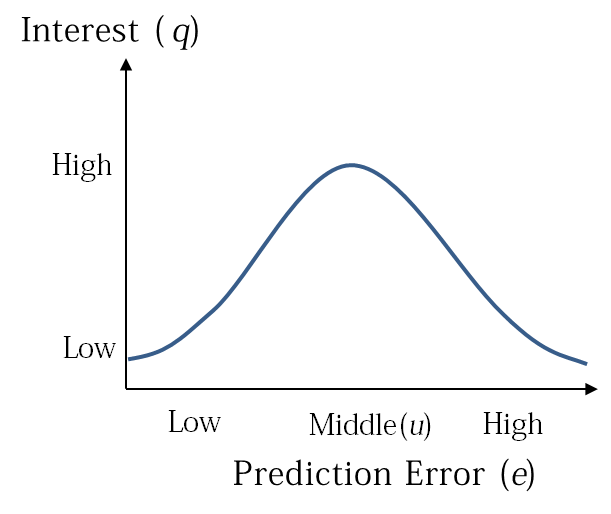
\includegraphics[width=0.45\textwidth,natwidth=700,natheight=450]{Figure5.png}
\caption{Visual attention module. a) Gaussian-shaped curve of interest value in function of the prediction error, b) Probability of looking away from the current visual position in function of the interest value.}
\label{Attention}
\end{figure}

\section{Experiments}

\subsection{Experimental settings}
In our experiment we reproduced similar experimental settings to those described in \cite{sommerville2005action}. We conducted simulated experiments with the simulated version of the humanoid robot iCub. The experiments consider two scenarios: the watch-first and the reach-first condition. For each experiment, the robot is placed 40 centimeters away of two objects, separated from each other by another 40 centimeters (see Fig. \ref{iCub}). In the watch-first scenario, the system first observes another individual reaching for one of the object from the same location as the robot; this phase is called the visual habituation. Then, the position of the objects is swapped and the system observes two more actions: reaching for the other object (new goal event) and reaching for the same object (new path event). In the reach-first scenario, the same process is repeated but this time the system experienced reaching for both objects in the action task, before the visual habituation. This experiment is depicted in Fig. \ref{experiment}.

\begin{figure*}
\centering
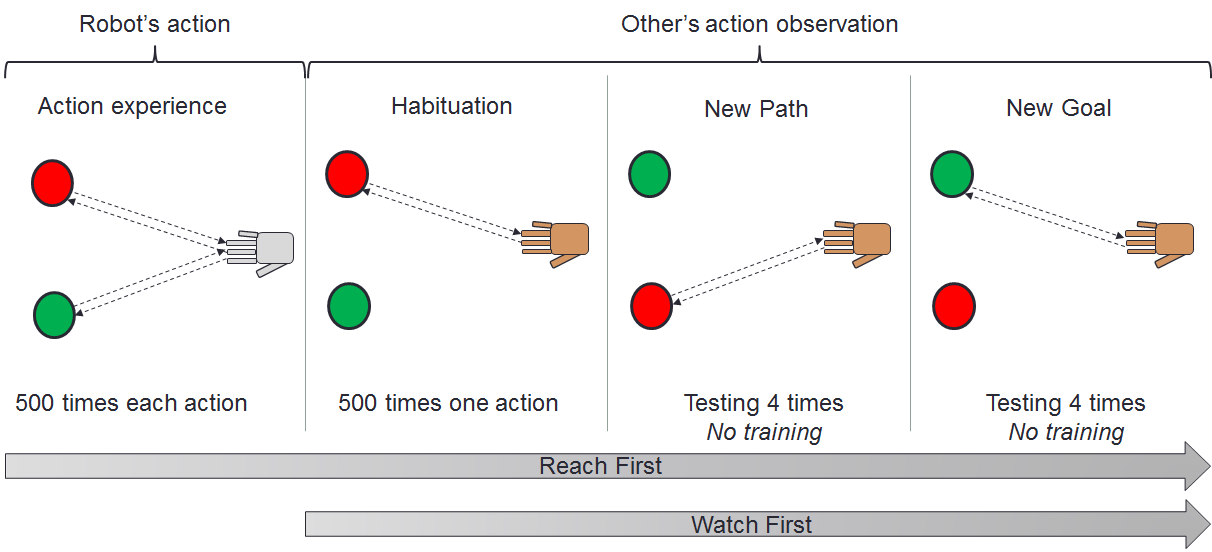
\includegraphics[width=0.9\textwidth,natwidth=700,natheight=450]{Figure2.png}
\caption{Procedure of the experiment}
\label{experiment}
\end{figure*}

\subsection{Action Task}
During the action task, the robot arm moved toward and touched one of two objects, then came back to the initial position and repeated the same action for the same or the other object randomly (see Fig. \ref{iCub}). This task corresponds to first stage of training for the reach-first condition. The neural network was trained with both vision and motor data of 500 reaching actions, where each action was trained for 175 learning iterations, which gives a total of 85000 learning steps. This training process was carried out for 20 trials. Fig. \ref{Error} (a) depicts the mean error of the action task over all training trials.

\begin{figure}
\centering
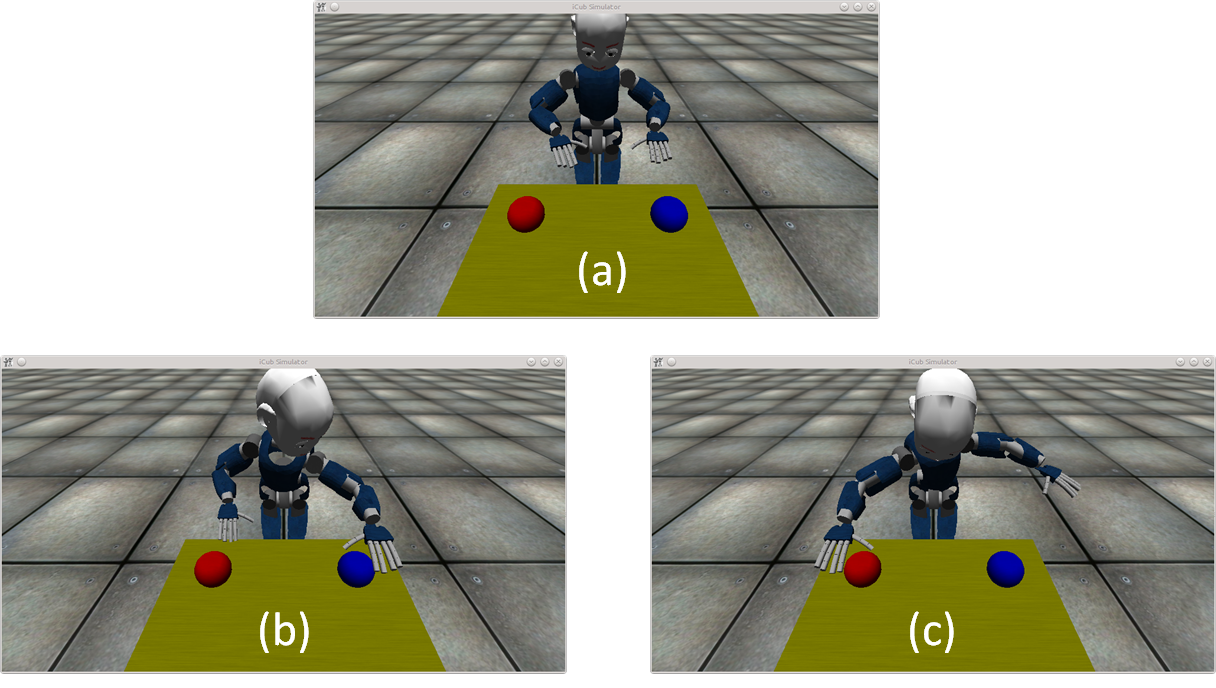
\includegraphics[width=0.45\textwidth,natwidth=700,natheight=450]{Simulator.png}
\caption{Experiment setting. (a): initial position before reaching; (b): reaching for object to the left of the robot; (c): reaching for object to the right of the robot.}
\label{iCub} 
\end{figure}

\subsection{Visual Habituation}
The visual habituation procedure consisted of training the neural networks with the visual data when observing reaching actions. For the reach-first scenario, the neural network was the same trained during the action task. We performed 500 visual habituations. Fig. \ref{Error} (b) and \ref{Error} (c) show the mean error curves for reach-first condition and watch first condition, respectively. For reference purpose, the prediction error corresponding to the condition without no experience (e.g., watch-first condition) of 0.365 was considered the maximum value of the prediction error. From the graphs we can observe that for both conditions there was an increase of the error in the first iteration. However, we can notice that the error for reach-first condition was 0.08, which is much lower than the error in watch-first condition. It means that visual information learned during the action task of the reach-first condition contributed to keep the error relatively low. Our interpretation of the result in the first habituation trial is that the lack of familiarity with the event caused an increase of prediction error, which in the case of the system with action experience (e.g., reach-first) was lower due to the visual experience of own actions. Fig. \ref{Error} plots the probability of looking away applying the principle of predictability (section III-D). The mean value \(\text{U}\) (Eq. \ref{gaussian}) used for the interest function \(\text{N}\) was defined as half of the maximum prediction error,The variance \(\sigma\) was arbitrarily defined to be 0.7 for illustration purposes, since it does not alter the relation between high and low errors \(\text{E}\)  and low and high probabilities \(\text{A}\). It must be notice that \(\sigma\) controls the magnitude of influence of the prediction error on the attention, and must be tuned for real implementations. Then, Fig \ref{Error} shows that the probability of looking away for reach-first condition was lower than the probability for watch-first condition.

In relation to the findings of Sommerville et al.\cite{sommerville2005action}, these results in the first habituation trial may explain why during the first habituation trial infants kept more attention compared to watch-first condition: the motor experience contributed to form a representation of own visual experience, which contributed to decrease the prediction error when observing others' actions and consequently to decrease the probability of looking away from an event.

\begin{figure}
\centering
%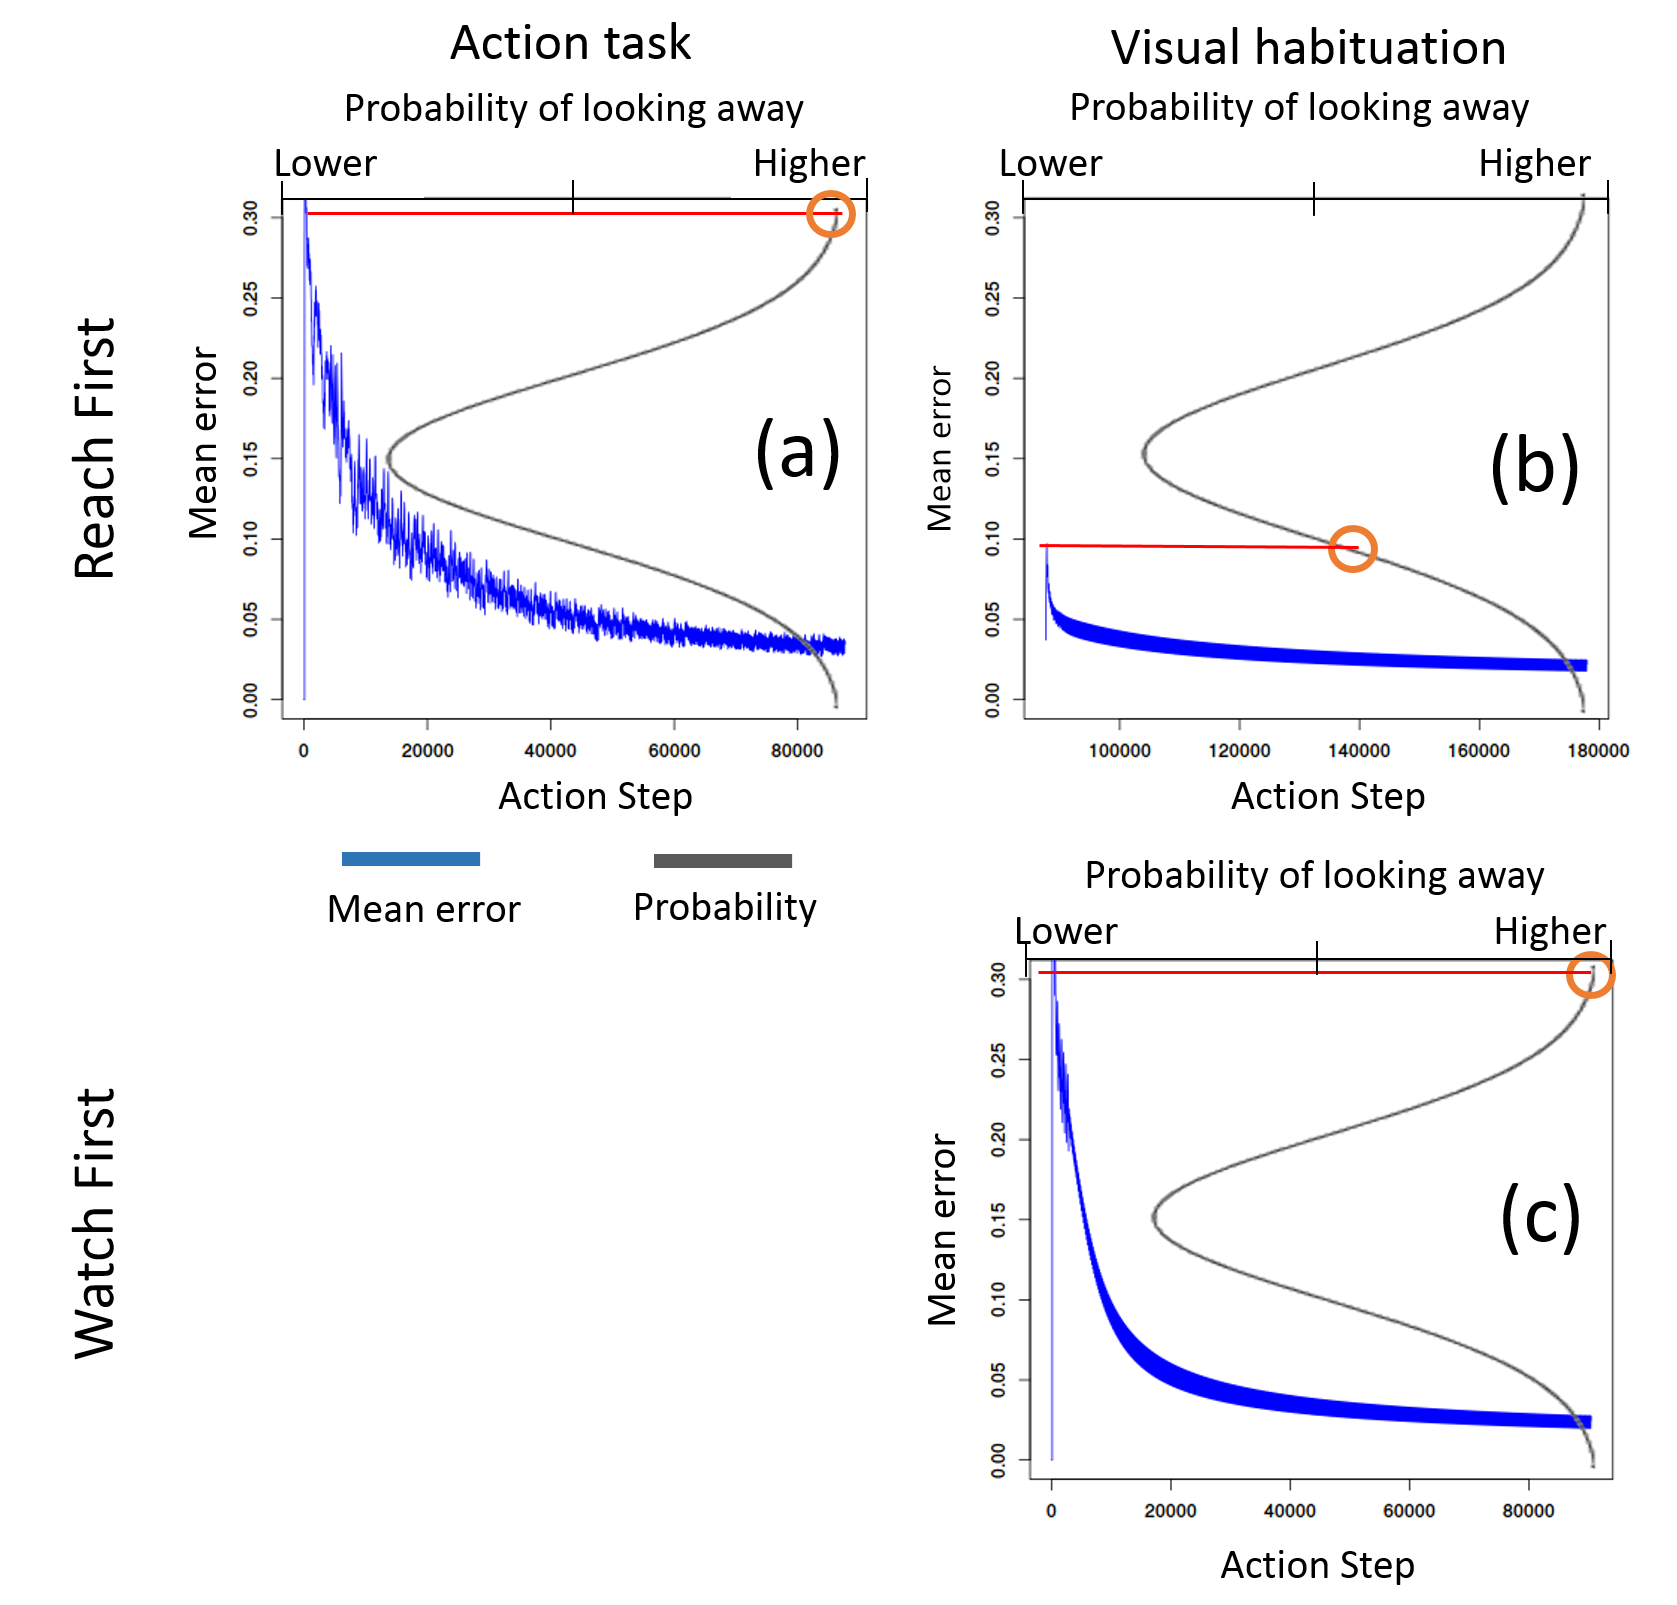
\includegraphics[width=0.5\textwidth,natwidth=700,natheight=450]{AT_HT_with_Attention.png}
\includegraphics[width=0.57\textwidth,natwidth=500,natheight=300,trim=80 100 0 100]{HAB_RESULT.eps}
\caption{Training of the neural network for watch-first condition and reach-first condition. The bottom horizontal axes represent the action step, the vertical axes represent the mean error and the top horizontal axes represent the probability of looking away. The blue line and the gray line are the mean error in function of the action step and the probability of looking away in function of the mean error, respectively. The red line and point represent the intersection of the mean error with the probability curve of looking away. (a) Mean error during action task for reach-first condition over all training trials; (b) Mean error and probability of looking away during habituation task for reach-first condition; (c) Mean error  and probability of looking away during habituation task for watch-first condition}
\label{Error}
\end{figure}

\subsection{New Path and New Goal}
After the networks were trained for both watch-first and reach-first conditions, we measured the visual prediction error when the goal or the trajectory were changed respect to the original action employed during the visual habituation, namely new goal and new path event. The graphs of the mean error and probability of looking away for watch-first condition and reach-first condition are shown in Fig. \ref{figure7}. From the graphs we can see that the change of path or goal produced an increase of the prediction error for all conditions in comparison with their values in the last phase of habituation. The results showed that for the system without motor experience (e.g., watch-first condition) the prediction error fluctuated in values more distant from the mean value \(\text{U}\) of the prediction error.  However, for the system with motor experience (e.g., reach-first condition) the prediction error took closer values to the mean value \(\text{U}\). Therefore, the increase of attention was higher for new goal and reach-first condition than for other conditions. An explanation for this result is that, while the experience of only visual information during the habituation may lead to a specific set of visual relations that can be subject to drastically changes, the visuomotor experience during action task may lead to a system that learns to represent patterns of actions based on own visuomotor experience and therefore is more robust to visual changes (e.g., the action of reaching an object is independent of the visual characteristics of the target). As a consequence, the system with visuomotor experience generates closer but not perfect predictions, which produces moderate prediction errors.

\begin{figure}
\centering
%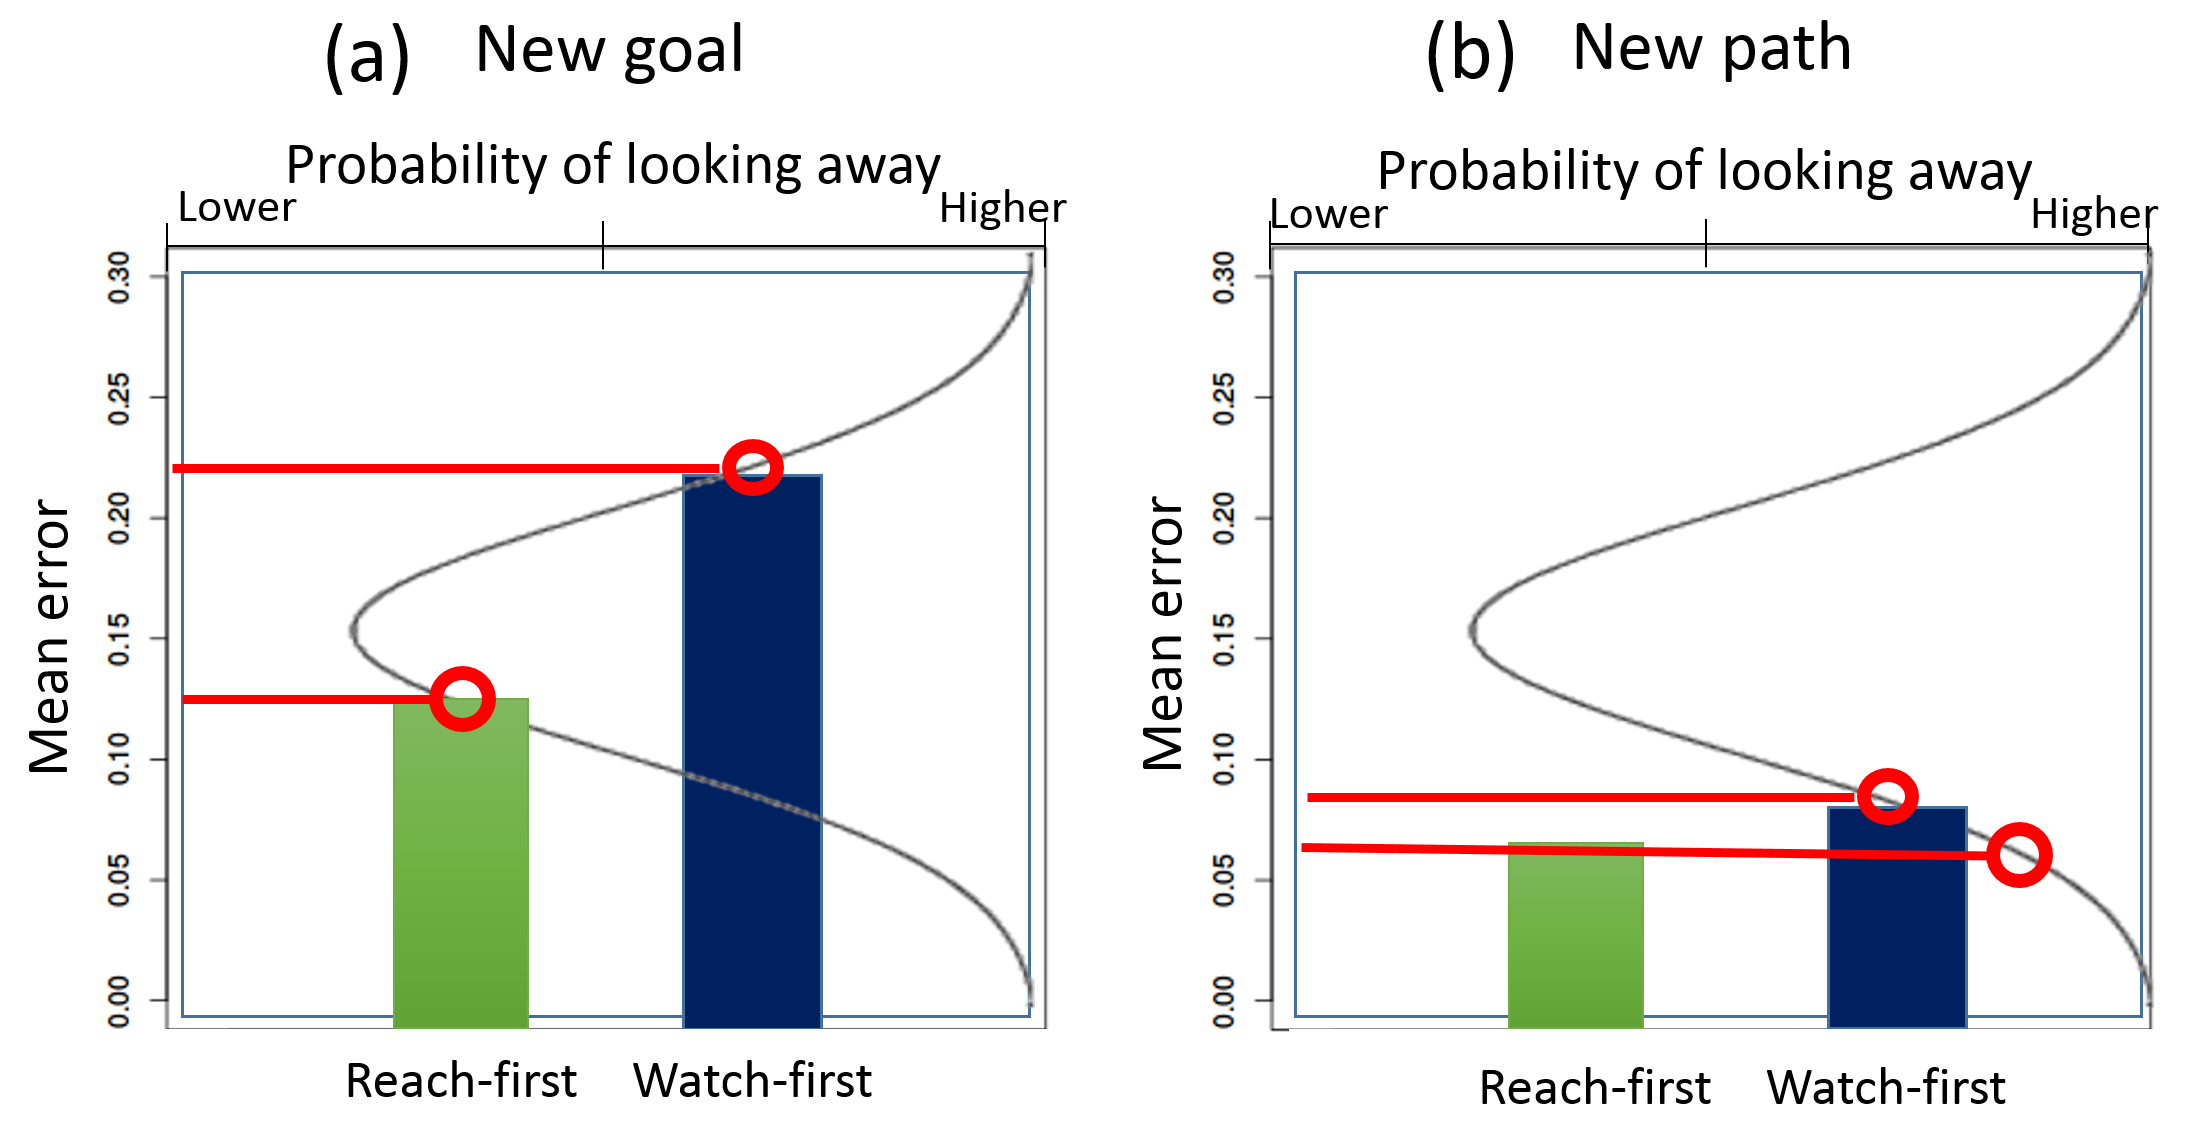
\includegraphics[width=0.5\textwidth,natwidth=700,natheight=450]{TT_with_Attention.png}
\includegraphics[width=0.48\textwidth,natwidth=500,natheight=300,trim=0 150 0 -50]{TEST_RESULT.eps}
%  \includegraphics[width=7cm,bb=0 0 400 500,trim=200 150 0 0]{TEST_RESULT.eps}
\caption{Error and probability of looking away during the test event. In both graphs the bottom horizontal axis represents the condition, the vertical axis represents the mean error and the top horizontal axis represents the probability of looking away. The green and blue bars represents the mean error for the reach-first condition and the reach-first condition, respectively. The gray line, whose independent axis is the top horizontal axis, represents the probability of looking away in function of the mean error. The red line and point represent the intersection of the mean error with the probability curve of looking away. (a) for new goal event, (b) Results for new path event.}
\label{figure7}
\end{figure}

\section{Discussion}
It should be noticed that from the experiments of Sommerville et al. \cite{sommerville2005action} we could not get measures in the habituation phase of the looking time of infants with interaction experience without gloves. We consider that getting that data will be useful to confirm, in terms of looking time, the quantitative difference between the influence of the motor and visual information of non-coordinated interactions and of coordinated interactions. Here we assumed that infants without gloves would perform similarly to infants under watch-first condition, since they cannot perform coordinated interactions and thus they can hardly learn useful information from their sensorimotor experience for prediction purposes.

Nonetheless, we consider that the results based on our computational approach bring important findings that may shed a light on the influence that the motor information has on the perception of others' actions. Our experimental results in the action task showed that the system was able to acquire a joint representation of visual and motor experience of coordinated interactions (i.e., reach-first condition), and in the visual habituation phase the system was able to apply that visuomotor experience to make predictions of the visual and motor components of others' actions. The results showed that the prediction error was closer to intermediate values when having interaction experience (i.e., reach-first condition) than when having no interaction experience (i.e., watch-first condition). Our interpretation of these results is that the system with coordinated visuomotor experience associates visual experience of own actions and visual information of others' actions, which can lead to generate a moderate prediction error that stimulates an increase of visual attention.

The test experiment for new path (same goal, different trajectory of the hand) and new goal (different goal, same trajectory of the hand) conditions tested the system after the habituation stage, where both systems (watch-first system and reach-first system) were already familiarized with the scene. The results showed the prediction error increased for both watch-first and reach-first conditions, but the prediction error for new goal (same path) under reach-first condition was closer to the intermediate error, which resulted in a higher attention, similarly to the experimental results described in \cite{sommerville2005action}. We attribute this result to the contribution of the motor component. During habituation in reach-first condition the system forms an association between its motor experience, including motion target, and the visual information of other's actions by using the joint visuomotor representation. Therefore, the visual information of others’ actions is employed to predict motor information of own experience, which influences the visual prediction. These prediction errors led to similar attention increases as reported by \cite{sommerville2005action}. Thus, the link between our computational results and the psychological findings is straightforward in terms of the strong connection between motor and sensory components, and the influence that own motor experience has on visual attention.

\section{Conclusion}
We proposed a computational model to explain psychological findings showing that action production alters the perception of other's actions \cite{sommerville2005action}. The experimental results showed that the influence of the motor experience on the joint representation of own visuomotor experience lead to changes in perception of others' actions. Our hypothesis proved to be valid to explain main findings relating the visuomotor experience and the allocation of visual attention in infants.

As a future work, we consider refining the representation of the motor and visual information and implementing the model in a real iCub platform. We believe that the prediction error may play a vital role not only in visual attention allocation but also in other domains at a cognitive level. We also find crucial to investigate the possible developmental connections between visual attention and prediction of others' actions, as recent psychological studies employing similar settings has shown that infants make distinctions between path and goal for prediction purposes \cite{cannon2012infants}.

\section*{Acknowledgment}
This work is partially supported by MEXT/JSPS KAKENHI (Research Project Numbers: 24119003, 24000012, 25700027) and JSPS Core-to-Core Program, A. Advanced Research Networks.

\bibliographystyle{ieeetr}
\bibliography{references}
\baselineskip 3.95mm

% An example of a floating figure using the graphicx package.
% Note that \label must occur AFTER (or within) \caption.
% For figures, \caption should occur after the \includegraphics.
% Note that IEEEtran v1.7 and later has special internal code that
% is designed to preserve the operation of \label within \caption
% even when the captionsoff option is in effect. However, because
% of issues like this, it may be the safest practice to put all your
% \label just after \caption rather than within \caption{}.
%
% Reminder: the "draftcls" or "draftclsnofoot", not "draft", class
% option should be used if it is desired that the figures are to be
% displayed while in draft mode.
%
%\begin{figure}[!t]
%\centering
%\includegraphics[width=2.5in]{myfigure}
% where an .eps filename suffix will be assumed under latex, 
% and a .pdf suffix will be assumed for pdflatex; or what has been declared
% via \DeclareGraphicsExtensions.
%\caption{Simulation Results}
%\label{fig_sim}
%\end{figure}

% Note that IEEE typically puts floats only at the top, even when this
% results in a large percentage of a column being occupied by floats.


% An example of a double column floating figure using two subfigures.
% (The subfig.sty package must be loaded for this to work.)
% The subfigure \label commands are set within each subfloat command, the
% \label for the overall figure must come after \caption.
% \hfil must be used as a separator to get equal spacing.
% The subfigure.sty package works much the same way, except \subfigure is
% used instead of \subfloat.
%
%\begin{figure*}[!t]
%\centerline{\subfloat[Case I]\includegraphics[width=2.5in]{subfigcase1}%
%\label{fig_first_case}}
%\hfil
%\subfloat[Case II]{\includegraphics[width=2.5in]{subfigcase2}%
%\label{fig_second_case}}}
%\caption{Simulation results}
%\label{fig_sim}
%\end{figure*}
%
% Note that often IEEE papers with subfigures do not employ subfigure
% captions (using the optional argument to \subfloat), but instead will
% reference/describe all of them (a), (b), etc., within the main caption.


% An example of a floating table. Note that, for IEEE style tables, the 
% \caption command should come BEFORE the table. Table text will default to
% \footnotesize as IEEE normally uses this smaller font for tables.
% The \label must come after \caption as always.
%
%\begin{table}[!t]
%% increase table row spacing, adjust to taste
%\renewcommand{\arraystretch}{1.3}
% if using array.sty, it might be a good idea to tweak the value of
% \extrarowheight as needed to properly center the text within the cells
%\caption{An Example of a Table}
%\label{table_example}
%\centering
%% Some packages, such as MDW tools, offer better commands for making tables
%% than the plain LaTeX2e tabular which is used here.
%\begin{tabular}{|c||c|}
%\hline
%One & Two\\
%\hline
%Three & Four\\
%\hline
%\end{tabular}
%\end{table}


% Note that IEEE does not put floats in the very first column - or typically
% anywhere on the first page for that matter. Also, in-text middle ("here")
% positioning is not used. Most IEEE journals/conferences use top floats
% exclusively. Note that, LaTeX2e, unlike IEEE journals/conferences, places
% footnotes above bottom floats. This can be corrected via the \fnbelowfloat
% command of the stfloats package.








% trigger a \newpage just before the given reference
% number - used to balance the columns on the last page
% adjust value as needed - may need to be readjusted if
% the document is modified later
%\IEEEtriggeratref{8}
% The "triggered" command can be changed if desired:
%\IEEEtriggercmd{\enlargethispage{-5in}}

% references section

% can use a bibliography generated by BibTeX as a .bbl file
% BibTeX documentation can be easily obtained at:
% http://www.ctan.org/tex-archive/biblio/bibtex/contrib/doc/
% The IEEEtran BibTeX style support page is at:
% http://www.michaelshell.org/tex/ieeetran/bibtex/
%\bibliographystyle{IEEEtran}
% argument is your BibTeX string definitions and bibliography database(s)
%\bibliography{IEEEabrv,../bib/paper}
%
% <OR> manually copy in the resultant .bbl file
% set second argument of \begin to the number of references
% (used to reserve space for the reference number labels box)
%\begin{thebibliography}{1}

%\bibitem{IEEEhowto:kopka}
%H.~Kopka and P.~W. Daly, \emph{A Guide to \LaTeX}, 3rd~ed.\hskip 1em plus
% 0.5em minus 0.4em\relax Harlow, England: Addison-Wesley, 1999.

%\end{thebibliography}




% that's all folks
\end{document}


